\chapter{多维随机变量及其分布}
\section{二维随机变量及其分布}
\subsection{二维随机变量}
\dfn{二维随机变量}{
    设随机试验的样本空间为$S$,定义在$S$上的实值单值函数$X = X(\omega)\;Y=Y(\omega)$为两个随机变量.称向量$(X,Y )$为定义在$S$上的\vocab{二维随机变量}
    \begin{center}
        i.e.    $\begin{aligned}
                X:S     & \to\RR   \\
                Y:S     & \to\RR   \\
                (X,Y):S & \to\RR[2]
            \end{aligned}$
    \end{center}
}
类似地,我们可以得到$n$维随机变量的定义.
\subsection{二维随机变量的分布函数}
\dfn{二维随机变量的分布函数}{
    设$(X,Y)$是二维随机变量,对于任意实数$x,y$,定义二元函数
    \begin{equation}
        F(x,y) = \Pr{X\leq x\cap Y\leq y} \defeq \Pr{X\leq x, Y\leq y}
    \end{equation}
    称为二维随机变量$(X,Y)$的\vocab{分布函数},或\vocab{联合分布函数(Joint CDF)}.
}
\begin{figure}[h]
    \centering
    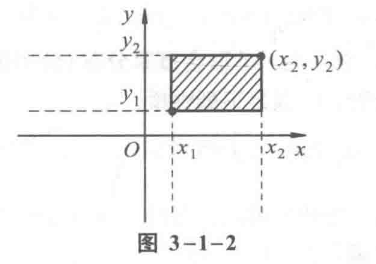
\includegraphics[scale=.6]{jointCDF}
    \caption{分布函数示意图}
\end{figure}
将这个向量视作平面内随机点的座标,分布函数就是随机点$(X,Y)$落入矩形域的概率.通过容斥原理,我们可以计算得到
\begin{equation}
    \Pr{x_1\leq X \leq x_2, y_1\leq Y\leq y_2} = F(x_2,y_2) - F(x_1,y_2) - F(x_2,y_1) + F(x_1,y_1)
\end{equation}
\subsubsection{联合CDF的性质}
\leftnote[1cm]{右侧几个等式可通过矩形域的面积来理解.}
\begin{enumerate}
    \item $0\leq F(x,y )\leq 1$
          \begin{enumerate}
              \item 固定$y$,$F(-\infty,y ) = 0$;
              \item 固定$x$,$F(x,-\infty) = 0$;
              \item $\lim_{\substack{x\to +\infty\\y\to +\infty}}F(x,y ) = 1, \lim_{\substack{x\to -\infty\\y\to -\infty}}F(x,y) = 0$
          \end{enumerate}
    \item (\textit{单调性})$F(x,y )$关于$x$和$y$都是单调不减的.
          \begin{enumerate}
              \item 固定$y$,$F(x,y )$关于$x$单调不减;
              \item 固定$x$,$F(x,y )$关于$y$单调不减.
          \end{enumerate}
    \item (\textit{连续性})$F(x,y )$关于$x$和$y$都是右连续的.
\end{enumerate}
若已知$(X,Y)$的分布函数$F(X,Y)$,则可由之导出各个参数(在固定另一个参数的情况下)各自的分布函数:
\begin{align}
    F_X(X) & = \Pr{X\leq x } =\Pr{X\leq x} = \lim_{y\to +\infty}F(x,y), \\
    F_Y(y) & = \Pr{Y\leq y } =\Pr{Y\leq y} = \lim_{x\to +\infty}F(x,y),
\end{align}
如此导出的CDF称为\vocab{边缘分布函数}.